\section{Number Theory}

This section develops the elementary arithmetic of the integers that underlies analytic number theory. Its organization follows the treatment of divisibility, prime factorization, arithmetic functions, and congruences in Apostol \cite[Chapters 1, 2, and 5]{Apostol1976-xj}. The discussion of residue classes also prepares the way for Dirichlet characters and $L$-functions, as in the course outline in \textit{Guia2}.

\subsection{Divisibility and the Greatest Common Divisor}

\begin{definition}[Divisibility]
For integers $a$ and $b$, with $a\ne 0$, we say that $a$ divides $b$, and write $a\mid b$, if there is an integer $q$ such that $b=aq$. In this case, $a$ is a divisor of $b$ and $b$ is a multiple of $a$.
\end{definition}

\begin{theorem}[Division algorithm]
For every integer $a$ and positive integer $b$, there are unique integers $q$ and $r$ such that
\[
 a=bq+r,\qquad 0\leq r<b.
\]
\end{theorem}

\begin{definition}[Greatest common divisor]
For integers $a$ and $b$ that are not both zero, the greatest common divisor $\gcd(a,b)$ is the unique positive integer $d$ that divides both $a$ and $b$ and is divisible by every common divisor of $a$ and $b$.
\end{definition}

\begin{theorem}[Euclidean algorithm and Bézout's identity]
For positive integers $a$ and $b$, repeated application of the division algorithm gives the Euclidean algorithm: divide successively, using each nonzero remainder as the next divisor. The last nonzero remainder is $\gcd(a,b)$. More generally, for integers $a,b$ that are not both zero, there exist integers $x,y$ such that
\[
 \gcd(a,b)=ax+by.
\]
\end{theorem}

\begin{proof}
At each division step, $r_{j-1}=q_jr_j+r_{j+1}$. A common divisor of $r_{j-1}$ and $r_j$ divides $r_{j+1}$, and a common divisor of $r_j$ and $r_{j+1}$ divides $r_{j-1}$. Thus consecutive pairs have the same common divisors, so the last nonzero remainder is the greatest common divisor. The remainders are integer linear combinations of the initial pair, by repeated substitution in the division equations. Consequently, the last nonzero remainder has the form $ax+by$. For integers of arbitrary sign, apply the algorithm to $|a|$ and $|b|$ and adjust the signs of the resulting coefficients; when one integer is zero, the identity follows directly.
\end{proof}

\begin{example}[Computing a greatest common divisor]
Applying the Euclidean algorithm gives
\begin{align*}
252&=1\cdot198+54,\\
198&=3\cdot54+36,\\
54&=1\cdot36+18,\\
36&=2\cdot18.
\end{align*}
Therefore, $\gcd(252,198)=18$. Back-substitution gives $18=4\cdot252-5\cdot198$, illustrating Bézout's identity.
\end{example}

\subsection{Prime Numbers and Unique Factorization}

\begin{definition}[Prime number]
An integer $p>1$ is prime if its only positive divisors are $1$ and $p$. An integer greater than $1$ that is not prime is composite.
\end{definition}

\begin{theorem}[Fundamental theorem of arithmetic]
Every integer $n>1$ is a product of primes, and this factorization is unique up to the order of its factors. Equivalently, it can be written uniquely as
\[
 n=\prod_{j=1}^{k}p_j^{\alpha_j},
\]
where $p_1<\cdots<p_k$ are primes and each $\alpha_j$ is a positive integer.
\end{theorem}

\begin{theorem}[Infinitude of primes]
There are infinitely many prime numbers.
\end{theorem}

\begin{proof}
Suppose that the complete list of primes were $p_1,\ldots,p_k$. The integer $N=p_1p_2\cdots p_k+1$ is greater than $1$, so it has a prime divisor. None of $p_1,\ldots,p_k$ divides $N$, since each leaves remainder $1$ upon division into $N$. This contradicts the assumption that the list contained every prime.
\end{proof}

\subsection{Congruences and Residue Classes}

\begin{definition}[Congruence]
Let $m$ be a positive integer. Integers $a$ and $b$ are congruent modulo $m$, written
\[
 a\equiv b\pmod m,
\]
if $m\mid(a-b)$.
\end{definition}

Congruence modulo $m$ is an equivalence relation on $\mathbb{Z}$. The equivalence class of $a$ is
\[
 [a]_m=\{a+qm:q\in\mathbb{Z}\},
\]
and the set of residue classes is
\[
 \mathbb{Z}/m\mathbb{Z}=\{[0]_m,[1]_m,\ldots,[m-1]_m\}.
\]
Addition and multiplication of residue classes are defined by $[a]_m+[b]_m=[a+b]_m$ and $[a]_m[b]_m=[ab]_m$. These operations do not depend on the chosen representatives.

\begin{theorem}[Solvability of a linear congruence]
The congruence $ax\equiv b\pmod m$ has an integer solution $x$ if and only if $\gcd(a,m)\mid b$.
\end{theorem}

\begin{proof}
The congruence is equivalent to an equation $ax-b=km$ for some integer $k$, or $ax+(-k)m=b$. Every integer linear combination of $a$ and $m$ is divisible by $d=\gcd(a,m)$, so a solution requires $d\mid b$. Conversely, if $d\mid b$, Bézout's identity gives integers $u,v$ with $au+mv=d$. Multiplying by $b/d$ yields $a(u b/d)+m(v b/d)=b$, so $x=u b/d$ solves the congruence.
\end{proof}

\subsection{Units and Euler's Totient Function}

A residue class $[a]_m$ has a multiplicative inverse modulo $m$ precisely when $\gcd(a,m)=1$. These invertible classes form the group of units $(\mathbb{Z}/m\mathbb{Z})^\times$ under multiplication.

\begin{definition}[Euler's totient function]
For a positive integer $m$, Euler's totient function is
\[
 \varphi(m)=\#\{a:1\leq a\leq m,\ \gcd(a,m)=1\}.
\]
Thus $\varphi(m)$ is the number of invertible residue classes modulo $m$.
\end{definition}

\begin{theorem}[Euler's theorem]
If $\gcd(a,m)=1$, then
\[
 a^{\varphi(m)}\equiv1\pmod m.
\]
\end{theorem}

\begin{proof}
Multiplication by $[a]_m$ permutes the invertible residue classes modulo $m$. Multiplying all classes in this permutation gives
\[
 [a]_m^{\varphi(m)}\prod_{\substack{1\leq r\leq m\\\gcd(r,m)=1}}[r]_m
 =\prod_{\substack{1\leq r\leq m\\\gcd(r,m)=1}}[r]_m.
\]
The product on the right is invertible, so it can be cancelled, yielding the claimed congruence.
\end{proof}

\begin{example}[Residue classes modulo $5$]
The classes modulo $5$ are $[0]_5,[1]_5,[2]_5,[3]_5,[4]_5$. The invertible classes are $[1]_5,[2]_5,[3]_5,[4]_5$, so $\varphi(5)=4$. For example, Euler's theorem gives $2^4\equiv1\pmod5$.
\end{example}

\begin{example}[A fully worked application modulo $12$]
For $m=12$, the greatest common divisors of the integers from $1$ to $12$ with $12$, in order, are
\[
 \bigl(\gcd(1,12),\gcd(2,12),\ldots,\gcd(12,12)\bigr)
 =(1,2,3,4,1,6,1,4,3,2,1,12).
\]
Hence the integers in this range that are relatively prime to $12$ are exactly $1,5,7,11$, and the totient value is
\[
 \varphi(12)=\#\{r:1\leq r\leq12,\ \gcd(r,12)=1\}
 =\#\{1,5,7,11\}=4.
\]
Equivalently, since the numbers not relatively prime to $12$ are those divisible by $2$ or $3$, inclusion--exclusion gives
\[
 \varphi(12)=12-\frac{12}{2}-\frac{12}{3}+\frac{12}{6}=4.
\]
Now take $a=5$. Since $\gcd(5,12)=1$, Euler's theorem applies, with exponent $\varphi(12)=4$. Direct calculation verifies the conclusion:
\[
 5^{\varphi(12)}=5^4=(5^2)^2=25^2=625=52\cdot12+1,
 \qquad\text{so}\qquad 5^4\equiv1\pmod{12}.
\]
\end{example}

The unit classes and their multiplicative characters are the algebraic starting point for Dirichlet $L$-functions, developed in a later section and in the course guide \textit{Guia2}.

\subsection{Divisors and Abundant Numbers}

\begin{definition}[Sum-of-divisors function]
For a positive integer $n$, define
\[
 \sigma(n)=\sum_{d\mid n}d,
\]
the sum of all positive divisors of $n$.
\end{definition}

\begin{theorem}[Formula for the sum of divisors]
If $n=\prod_{j=1}^{k}p_j^{\alpha_j}$ is the prime factorization of $n$, then
\[
 \sigma(n)=\prod_{j=1}^{k}\left(1+p_j+p_j^2+\cdots+p_j^{\alpha_j}\right)
 =\prod_{j=1}^{k}\frac{p_j^{\alpha_j+1}-1}{p_j-1}.
\]
\end{theorem}

\begin{proof}
Every positive divisor of $n$ is obtained by choosing, independently for each prime $p_j$, an exponent from $0$ to $\alpha_j$. Summing the resulting products over all choices factors into the product of the geometric sums shown above.
\end{proof}

\begin{definition}[Abundant number]
A positive integer $n$ is abundant if the sum of its proper positive divisors is greater than $n$. Since the proper divisors omit $n$ itself, this is equivalent to $\sigma(n)>2n$.
\end{definition}

\begin{example}
The positive divisors of $12$ are $1,2,3,4,6,12$. Their sum is $\sigma(12)=28$, and the proper divisors sum to $1+2+3+4+6=16>12$. Thus $12$ is abundant.
\end{example}

\subsection{A First Look at the Distribution of Primes}

\begin{definition}[Prime-counting function]
For real $x\geq2$, let
\[
 \pi(x)=\#\{p\leq x:p\text{ is prime}\}.
\]
\end{definition}

\begin{theorem}[Prime number theorem]
\[
 \pi(x)\sim\frac{x}{\log x}\qquad(x\to\infty),
\]
\end{theorem}

Here $f(x)\sim g(x)$ means that $f(x)/g(x)\to1$. This asymptotic description is one of the central results of analytic number theory; its proof is deferred to the later study of prime distribution \cite[Chapter 4]{Apostol1976-xj}.
\begin{figure}[H]
\centering
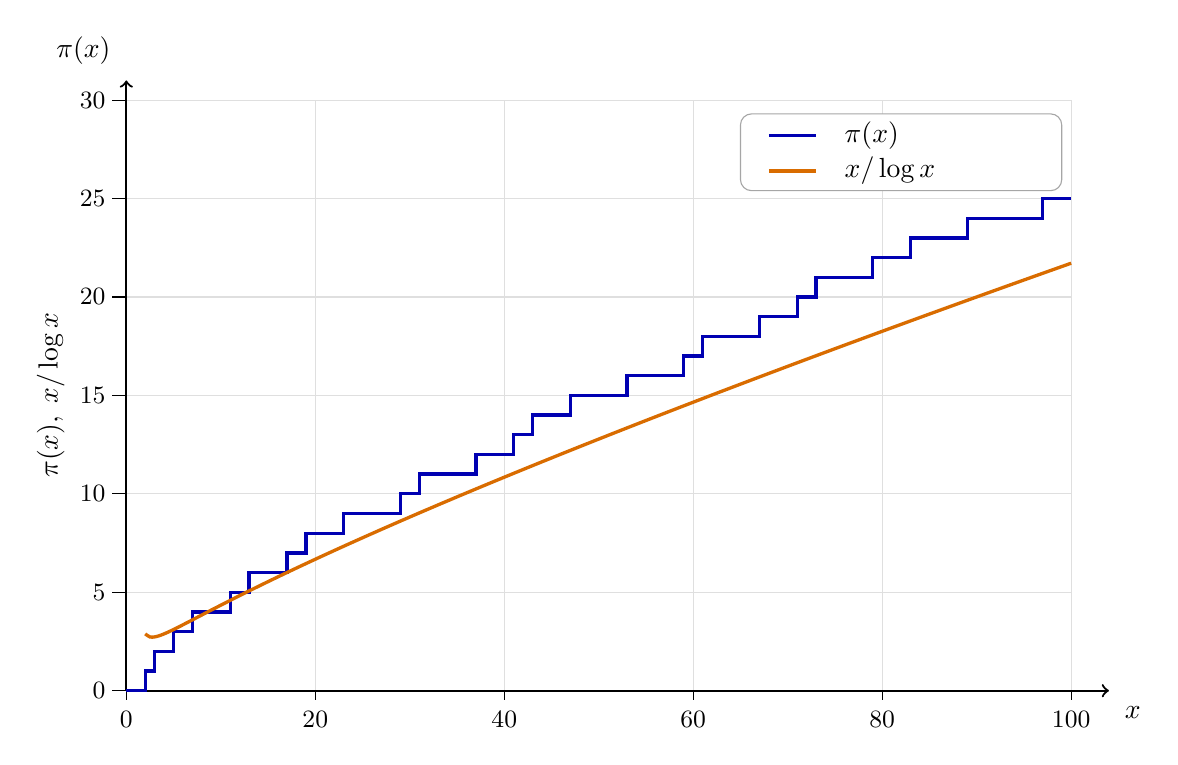
\begin{tikzpicture}[x=0.12cm,y=0.25cm]
    \foreach \x in {0,20,...,100} {
        \draw[gray!25,thin] (\x,0) -- (\x,30);
        \draw[black] (\x,0) -- (\x,-0.45);
        \node[below=4pt] at (\x,0) {\small \x};
    }
    \foreach \y in {0,5,...,30} {
        \draw[gray!25,thin] (0,\y) -- (100,\y);
        \draw[black] (0,\y) -- (-1.5,\y);
        \node[left=4pt] at (0,\y) {\small \y};
    }

    \draw[->,thick] (0,0) -- (104,0) node[below right=2pt] {$x$};
    \draw[->,thick] (0,0) -- (0,31) node[above left=2pt] {$\pi(x)$};
    \node[rotate=90] at (-8,15) {$\pi(x),\;x/\log x$};

    \draw[blue!70!black,very thick]
        (0,0) -- (2,0) -- (2,1) -- (3,1) -- (3,2) -- (5,2) -- (5,3)
        -- (7,3) -- (7,4) -- (11,4) -- (11,5) -- (13,5) -- (13,6)
        -- (17,6) -- (17,7) -- (19,7) -- (19,8) -- (23,8) -- (23,9)
        -- (29,9) -- (29,10) -- (31,10) -- (31,11) -- (37,11) -- (37,12)
        -- (41,12) -- (41,13) -- (43,13) -- (43,14) -- (47,14) -- (47,15)
        -- (53,15) -- (53,16) -- (59,16) -- (59,17) -- (61,17) -- (61,18)
        -- (67,18) -- (67,19) -- (71,19) -- (71,20) -- (73,20) -- (73,21)
        -- (79,21) -- (79,22) -- (83,22) -- (83,23) -- (89,23) -- (89,24)
        -- (97,24) -- (97,25) -- (100,25);

    \draw[orange!85!black,very thick,samples=200,domain=2:100,smooth,variable=\x]
        plot (\x,{\x/ln(\x)});

    \path[fill=white,draw=black!35,rounded corners] (65,25.4) rectangle (99,29.3);
    \draw[blue!70!black,very thick] (68,28.2) -- (73,28.2);
    \node[anchor=west] at (75,28.2) {$\pi(x)$};
    \draw[orange!85!black,very thick] (68,26.4) -- (73,26.4);
    \node[anchor=west] at (75,26.4) {$x/\log x$};
\end{tikzpicture}
\caption{The prime-counting function $\pi(x)$ and its asymptotic comparison $x/\log x$ on $2\leq x\leq100$.}
\label{fig:prime-number-theorem}
\end{figure}

The plot illustrates the prime number theorem on a finite interval; the asymptotic equivalence concerns the limit as $x\to\infty$ and is not established by this graph.